\subsection{Topic Modelling}\label{subsec:topicModelling}
The objective of topic modelling is to infer topics (collections of words) in a document set.
The result consists of a topic-word distribution matrix $\varphi$, which for each topic gives a distribution of words belonging to said topic, and a document-topic distribution matrix $\theta$ which for each document gives a distribution of topics to which the document belongs to.

\subsubsection{\acrlong{LDA}}\label{subsec:lda}
\todo{cite lda} introduce \gls{LDA}, which has since become a staple within topic modelling.
\gls{LDA} works under the assumption that documents are generated from a specific generative process, and then tries to reverse engineer this process.
This process generates $K$ topics and $M$ documents containing $N_{i\dots M}$ words.
This generative process assumes that documents are random mixtures of latent topics and that each topic is a distribution over all the words in the corpus.
The generative process have two dirichlet distributions $Dir(\alpha)$ for the document-topic relation and $Dir(\beta)$ for the topic-word relation.

\begin{figure}[h]
	\centering
	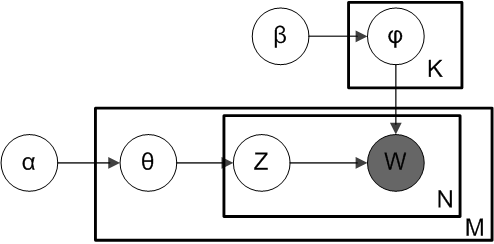
\includegraphics[width= 0.3 \textwidth]{figures/Smoothed_LDA.PNG}
	\caption{Plate notation for \gls{LDA}. Boxes symbolize repeated processes, shaded elements are observed information. Image is from \url{https://en.wikipedia.org/wiki/Latent_Dirichlet_allocation}}
	\label{fig:lda}
\end{figure}

From these dirichlets, we can sample two multinomial distributions: document-topic $\theta$ and topic-word $\varphi$.
These dirichlets are tuned with the hyperparameters $\alpha$ and $\beta$, which adjust the entropy of the sampled distributions.
An $\alpha$ value near one causes each document to be distributed over almost all topics, while a $\alpha$ value near 0 causes each document to be distributed over only a few topics.
Similarly $\beta$ will adjust how many words each topic contains.
This also has the added consequence that a high $\alpha$ will make documents appear more similar, and a high $\beta$ will make topics appear more similar.

Using $\theta$ and $\varphi$ we can sample concrete topics $Z$ from documents, and concrete words $W$ from topics.
\autoref{fig:lda} gives an overview of the assumed generative process.
